\documentclass[12pt,fleqn]{article}\usepackage{../common}
\begin{document}
Ders 21

Bu ozdeger/vektorler hakkindaki ilk dersimiz. Bu degerler ozel
buyukluklerdir, ozel sayilardir, ve onlari niye istedigimizi, niye
hesapladigimizi gorecegiz.

Ozvektor nedir? 

Elimde bir $A$ matrisi var. Bir matris ne yapar? Vektorler uzerinde, mesela
$x$ vektoru, etkide bulunabilir, onlari degistirebilir. Sanki $A$'yi bir
fonksiyon gibi de gorebiliriz, $x$ vektoru $A$'ya ``giriyor'' ve
``disariya'' bir $Ax$ cikiyor. Calculus'ta oldugu gibi $f()$'e bir tek sayi
$x$ veriliyor, $f(x)$ geri disari cikiyor [hakikaten de $x$ ve $Ax$ ayni
boyutta yani giris cikis analojisi cok uygun]. Lineer Cebirde daha cok
boyut var, giren ve cikan vektorler.

Bu derste ozellikle ilgilendigim vektorler ise disari ciktigi zaman girdigi
haliyle {\em ayni yonu gosteren} vektorler. Dikkat, ``ayni'' olan vektorler
degil cikinca ayni ``yonu'' gosteren vektorler. Bu tipik bir durum olmazdi
degil mi? Cogunlukla $A$'yi bir uyguladik mi disari cikan vektor tamamen
baska bir yonu gosterir. Bizim ilgilendigimiz durumda oyle olmayacak, bu
durumda $Ax$, $x$'e paralel olacak. Iste bu vektorler ozvektorler olacak. 

Paralel ne demektir? Formulle daha rahat belirtilir,

$$ Ax = \lambda x $$

$\lambda$, yani ozdeger, bir skalardir. Iki tarafta $x$'in olmasi
paralellige isaret ediyor, sadece buyukluk ($\lambda$ uzerinden) degisik
olabiliyor. Tabii buyukluk derken $\lambda$ eksi degerde olabilecegi icin
vektorun ters yonde olmasina da izin vermis oluyoruz. $\lambda$ sifir da
olabilir, hatta hayali sayi bile olabilir.

Ozdeger sifir uzerinde biraz daha duralim. Bu durumda $Ax = 0 \cdot x$ elde
ederiz yani $Ax = 0$. Bu ne demektir? $x$'lerin $A$'nin null uzayinda
(nullspace) olmasi... Eger $A$ tekil (singular) ise, ki $Ax = 0$ bu demek
zaten demek ki oyle bir $x$ olabiliyor ki $Ax = 0$ olabiliyor, o zaman $x$
sifir olmayan bir vektordur, ve $\lambda = 0$ bir ozdeger olmalidir.

Bir projeksiyon matrisine bakalim, mesela $P$. Elimizde bir satih (plane)
var, ve bu sathin uzerinde yansitma yapan bir $P$ var. 

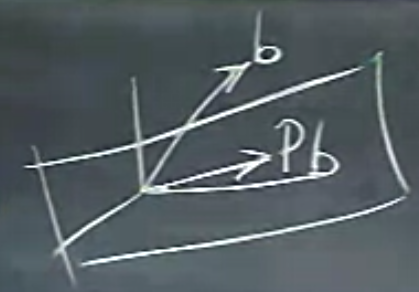
\includegraphics[height=4cm]{21_1.png}

$b$, $P$'nin bir ozvektoru mudur? Degildir. Cunku $b$ ve $Pb$ ayni yonu
gostermiyorlar. 

Peki, bu resme gore, yansitma sonrasi ayni yonde olacak bir vektor var
midir? Varsa nerededir? Cevap, eger $x$ ustteki duzlemin tam uzerinde ise
$P$ yansitmasi sonrasi ayni yonde kalir. Tabii yansitma tekrar kendisini
verir, yani vektor hic degismemis olur. $Px = x$, ki $\lambda = 1$.

Baska bir ozvektor var mi? Olmasini umuyorum cunku 3 boyuttayim ve bu
demektir ki 2 tane daha birbirinden bagimsiz ozvektor bulabilmeliyim, ki
nihayetinde ozvektorlerin ikisi duzlem uzerinde [duzlem iki boyutlu bir sey
olduguna gore), o zaman ucuncusu duzlem disinda olacak. Duzlem disinda olan
ozvektor dik olan ozvektor olmali.

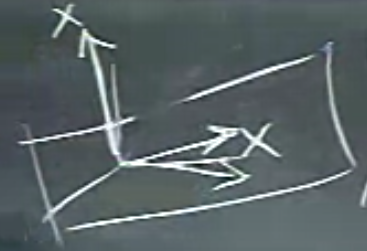
\includegraphics[height=4cm]{21_2.png}

Bu durumda $Px = 0$, ve $\lambda = 0$, cunku dikligin bir diger tanimi
carpim sonrasi sonucun sifir olmasi. 

Bir diger ornek. Su permutasyon matrisine bakalim. 

$$ 
A = \left[\begin{array}{cc}
0 & 1 \\
1 & 0
\end{array}\right]
 $$

 Bu matrisi hangi vektor ile carparsam ayni yonde bir vektor elde ederim?
 Permutasyon matrisi tanim itibariyle permutasyon yapar, yani ogelerin
 yerini degistirir. Iki boyut baglaminda bir vektorun iki ogesinin yerini
 degistirecektir. Peki hangi vektorun ogeleri yer degistirirse yine kendisi
 olur? Cevap basit, $x = [1 \ 1]$. 

$$ 
x = \left[\begin{array}{c}
1 \\ 1
\end{array}\right], 
Ax = \left[\begin{array}{c}
1 \\ 1
\end{array}\right], 
\lambda = 1, Ax = x
 $$

Bir tane daha ozdeger/vektor lazim. Bu diger ozdeger $\lambda = -1$
olmali. Peki nasil bir vektor olmali ki ogeleri yer degistirince ters yonu
gostersin? 

$$ 
x = \left[\begin{array}{r}
-1 \\ 1
\end{array}\right], 
Ax = \left[\begin{array}{r}
1 \\ -1
\end{array}\right], 
\lambda = -1, Ax = -x
 $$

Ozvektor/degerler hakkinda ufak bir sey daha soylemek istiyorum. $N \times
N$ matrisinin $N$ tane ozdegeri vardir. Bu degerleri bulmak kolay
degildir. 1., 2., hatta $N^{inci}$ seviye bir denklemden cikar bu
degerler. Fakat bize yardim eden bir numara vardir, tum ozdegerlerin
toplami matrisin kosegen degerlerinin toplamina esittir, ki bu toplama
``iz'' (trace) ismi verilir. 

Bu numarayi ustteki ornekte kullanirsak, $\lambda = 1$ buldugum anda diger
ozdegerin -1 oldugunu hemen bilirim, cunku ana matrisin izi sifir, 
$0 - 1 =
-1$. 

Artik ozdeger/vektor hesabina gelelim. $Ax = \lambda x$ denklemi var, bu
denklemde iki bilinmeyen var. Bu denklemi nasil cozerim? Bir numara, her
seyi tek terafa gonderirim,

$$ (A-\lambda I )x = 0 $$

Simdi bu denklem bana bir seyler soyluyor. Eger bir $x$ ``var'' ise, bu
varlik, $A-\lambda I$'nin tekil oldugu anlamina gelir. Peki tekil matrisler
hakkinda ne biliyorum? Determinantlarinin sifir oldugunu biliyorum. Yani,

$$ \det (A -\lambda I) = 0 $$

Bu denklem ozdeger denklemi, ya da karakteristik denklem (characteristic
equation) olarak bilinir. 

Ilk once $\lambda$ bulmakla ise baslarim. Tabii $N$ tane $\lambda$
olacaktir, bunlarin hepsini bulmakla ise baslarim. Not: $N$ $\lambda$
olmasi demek $N$ degisik $\lambda$ olmasi anlamina gelmiyor, bazi $\lambda$
degerleri kendini tekrar edebilir. Tabii tekrarlanan $\lambda$ bizim
dersteki her turlu derdin kaynagidir [biraz saka biraz gercek havasiyla
soyluyor hoca].

$\lambda$'yi bulunca ne yaparim? Matrisin null uzayini hesaplarim, ki artik
bu islemde usta olduk, eliminasyona baslarim, pivot bulurum, vs. 

Ornek

$$ 
A = \left[\begin{array}{ccc}
3 & 1 \\ 1 & 3
\end{array}\right]
 $$

Bu matris simetrik. Bu tur ozel sartlar matrisin ozdegerlerinin de ozel
olmasi  anlamina gelir. Mesela simetrik matrislerin tum ozdegerlerinin reel
sayi oldugunu hemen bilirim. Peki ozvektorler? Birbirlerine dik
olurlar. Bir onceki ornegi hatirlarsak, $[1 \ -1]$ ve $[-1 \ 1]$. 

$$ 
\det (A -\lambda I) = 
\left[\begin{array}{ccc}
3-\lambda & 1 \\ 
1 & 3-\lambda
\end{array}\right] = 
(3-\lambda)^2 -1 = 0
$$

$$ \lambda^2 - 6\lambda + 8 = 0 $$

Bu formuldeki $6$ nedir? Matris izinin eksi hali. Peki 8? O da
determinant. Yani 2x2 durumunda sayilar cok basit sekilde ortaya
cikiyorlar. Neyse, ustteki formulu faktorize edelim, $(\lambda - 4)(\lambda
- 2)$, 
yani $\lambda_1 = 4,\lambda_2 = 2$. 

Simdi ozvektorler: Bu vektorler kosegenden 2 ya da 4 cikartildigi zaman
ortaya cikan matrislerin null uzayidir. 

$$ 
\left[\begin{array}{ccc}
3-4 & 1 \\ 1 & 3-4
\end{array}\right] = 
\left[\begin{array}{ccc}
-1 & 1 \\ 1 & -1
\end{array}\right]
 $$

Bu matris tekil mi? Oyle. Bu matrisi $x_1 = [1 \ 1]$ ile carparsam sifir elde
ederim. Digeri?

$$ 
\left[\begin{array}{ccc}
3-2 & 1 \\ 1 & 3-2
\end{array}\right] = 
\left[\begin{array}{ccc}
1 & 1 \\ 1 & 1
\end{array}\right]
 $$

$x_2 = [1 \ -1]$. Bu da ikinci ozvektor.

Ilginc bir durum, bu sonuc permutasyon matrisinden gelen sonuca cok
benziyor. Fark nerede? Ana matrisin kosegenine 3 eklenmis, ya da $A + 3I$
yapilmis. Bunu yapinca ozdegerlere 3 eklemis oldum. Ama ozvektorler hic
degismeden kaldi.

Daha cetrefil bir ornek gorelim. Diyelim ki iki matris $A,B$'nin
ozdegerlerini biliyorum. $A+B$'nin ozdegerleri $\lambda,\alpha$ nedir?  Ilk
akla gelen cevap ``ozdegerleri toplanir'' dogru degil. Cunku

$$ (A+B)x = (\lambda+\alpha)x $$

demis oluruz, ama bunu derken ozvektorler ayni demis oluruz. Bu dogru
degildir. $A \cdot B$ ayni sekilde. Bunlar kotu ornekler. 

Bir ornek daha yapalim, bu sefer rotasyon matrisi. 90 derece dondurme
matrisi olsun.

Ornek

$$ Q =  
\left[\begin{array}{ccc}
\cos 90 & -\sin 90 \\
\sin 90 & \cos 90
\end{array}\right]
= \left[\begin{array}{ccc}
0 & -1\\
1  & 0
\end{array}\right]
$$

Bu bir dik, ortagonal bir matris. Ozdegerlerin toplami sifir olacak, cunku
iz oyle. Determinant ozdegerlerin carpimina esit, yani bu carpim 1 olacak. 

Fakat bu ornekte bazi seyler yanlis gidecek. Niye? Dusunelim, hangi vektor
bu matrise verilince, donduruldukten snora, disari ayni yonde olarak cikar?
Ozellikle 90 derece donduruldukten sonra. Gordugunuz gibi problem
cikabilir.  Ozdegerler ile de problem var, toplami 0 olan ama carpimi 1
olan nasil sayilar bulabilecegiz ki?

Fakat bir care var. Hesaplayalim, 

$$ \det(Q - \lambda I) = 
\left[\begin{array}{ccc}
-\lambda & -1 \\
1 & -\lambda
\end{array}\right] = \lambda^2 + 1 = 0
 $$

Ozdegerler nedir? $\lambda_1 = i, \lambda_2 = -i$. Bu sayilar kompleks / hayali
sayilardir, reel degillerdir. Bu olabilir. Bir matris, ustte oldugu gibi,
tamamen reel sayilardan olusabilir, ama ozdegerleri hayali olabilir. 

Bu iki hayali sayi birbirinin kopmleks eslenigi (complex
conjugate). Kompleks eslenigin ne oldugunu hatirliyoruz herhalde, bir
sayinin hayali kisminin isaretini degistirince onun kompleks eslenigini
elde etmis olurum. Ustteki sayilar zaten tamamen hayali bolumden olusuyor,
hic reel kisimlari yok, o tek kismin da isaretini degistirince eslenigi
elde ediyorum. 

Eger matrisim simetrik, ya da ``simetrige yakin'' olsaydi, ustteki durum
kesinlikle ortaya cikmazdi. Cunku kural odur ki, simetrik matrislerin
ozdegerleri reeldir. 

Bol bol ornek veriyorum ki tum olasiliklari gorebilelim. 

Bir kotu ihtimal daha.

$$ A = 
\left[\begin{array}{ccc}
3 & 1 \\ 0 & 3
\end{array}\right]
 $$

Bu matris ucgensel (triangular). Bu tur matrislerde ozdegerler kosegenin
uzerindedir! Bunu bilmek oldukca faydalidir. Ama kontrol edelim,

$$ \det(Q - \lambda I) = 
\left[\begin{array}{ccc}
3-\lambda & 1 \\
0 & 3-\lambda
\end{array}\right] = (3-\lambda)(3-\lambda) = 0, 
\lambda_1 = 3, \lambda_2 = 3
 $$

Problem nerede? Problem ozvektorlerde. Hatirlayalim, 

$$ (A-\lambda I)x = 0$$

denklemini cozuyoruz, yani

$$ (A-\lambda I)x = 
\left[\begin{array}{cc}
0 & 1 \\ 
0 & 0
\end{array}\right]
\vec{x}
=
\left[\begin{array}{c}
0 \\ 0
\end{array}\right]
$$

Burada $\vec{x}$ sonucunu ariyorum, bir vektor. Kafadan hemen birinci
ozvektoru bulabilirim, 

$$ x_1 = \left[\begin{array}{c}
1 \\ 0
\end{array}\right] $$

Peki ikinci ozvektor nedir? Bu vektorun birinciden bagimsiz olmasi gerekir,
unutmayalim. Boyle bir vektor bulabilir miyiz? Bulamayiz. Mumkun degil. Bu
sebeple bu ornege dejenere durum (degenerate case) denir. Ikinci bir
bagimsiz ozvektor yoktur. 

Ekler 

Alttaki anlatim alternatif bir kaynaktan alinmistir

Ozvektorler, Ozdegerleri Elle Hesaplamak (Eigenvectors, Eigenvalues)

Ozdegerler ve ozvektorler her matrise gore ozel vektorlerdir, ki matris bu
ozel vektorleri transform ettiginde / islediginde sonuc yine ozvektorun
kendisidir, daha dogrusu onun bir sabit (ozdeger) ile carpilmis
halidir. Yani

\[ Ax = \lambda x \]

Tek tarafa gecirelim

\[ Ax - \lambda x = 0 \]

Bu noktada $x$'leri disari cekmek isterdik, fakat bunu yapamayiz, cunku o
zaman iceride $A - \lambda$ kalir ve bu olmaz, cunku $A$ bir matris,
$\lambda$ bir tek sayi. Ama $Ix = x$'ten hareketle

\[ Ax - \lambda I x = 0 \]

diyebiliriz. Simdi disari cekersek

\[ (A - \lambda I) x = 0 \]

Bu ifadenin dogru olmasi icin parantez icindeki ifade / matris tekil
(singular) olmalidir. Bunun icin ise parantez icinin determinanti sifir
olmalidir. Yani

\[ |A - \lambda I| = 0 \]

Ornek 

\[ 
A = 
\left[\begin{array}{rr}
1 & 4 \\ 3 & 5
\end{array}\right]
 \]

\[ 
A - \lambda I = 
\left[\begin{array}{rr}
1 & 4 \\ 3 & 5
\end{array}\right] - 
\lambda
\left[\begin{array}{rr}
1 & 0 \\ 0 & 1
\end{array}\right] 
 \]

\[ 
= 
\left[\begin{array}{rr}
1 - \lambda & 4 \\ 3 & 5-\lambda
\end{array}\right]
 \]

\[ det(A - \lambda I) = (1-\lambda)(5-\lambda) - 4 \cdot 3 \]

Ustteki denkleme karakteristik denklem (characteristic equation) denir. 

\[ = -7 -6\lambda + \lambda^2 \]

Kokleri $\lambda_1 = 7$, $\lambda_2 = -1$.

Her ozdegere tekabul eden ozvektoru bulmak istiyorsak, cikartma islemini
yapalim

\[ 
A - \lambda I = 
\left[\begin{array}{rr}
1-7 & 4 \\ 3 & 5-7
\end{array}\right] = 
\left[\begin{array}{rr}
-6 & 4 \\ 3 & -2
\end{array}\right]
 \]

Su formule donersek

\[ (A - \lambda I) x = 0 \]

Cikartma sonrasi elimize gecen matrisi carpacak oyle bir $x$ vektoru
ariyoruz ki bu vektorle carpinca elimize sifir (vektoru) gecsin. Yani bu
aradigimiz $x$ vektoru $(A - \lambda I)$'nin sifir uzayinda (nullspace). 

2 x 2 boyutundaki boyle ufak bir ornek icin $x$'i aslinda tahmin
edebiliriz. Oyle iki sayi bulalim ki, 1. ve 2. kolonu onlarla ayri ayri
carpip topladigimizda sonuc sifir olsun. Her iki kolonun tepesinde -6 ve 4
goruyorum, sadece bu iki sayinin sifira toplanmasi icin acaba -6'yi 2 ile
4'u 3 ile carpip toplasam olur mu? Kolondaki diger sayilara bakiyoruz, 3 ve
-2 icin de bu ise yariyor. Demek ki ozvektorlerden biri 

\[ x_1 = 
\left[\begin{array}{r}
2 \\ 3
\end{array}\right]
 \]

Digeri ise, ayni teknigi kullanarak,

\[ x_2 = 
\left[\begin{array}{r}
-2 \\ 1
\end{array}\right]
 \]

Ekler

Ozdeger/Vektor Hesabinda Ust Metot (Power Method)

Diyelim ki bir $A$ matrisinin, ki $A \in \mathbb{R}^{n \times n}$,
ozdegerleri $\lambda_1,...,\lambda_n$ ve ozvektorleri $v_1,..,v_n$ olarak
verilmis. Bu demektir ki her $i=1,..,n$ icin $Av_i = \lambda_i v_i$.

Farzedelim ki bu matrisin tum ozvektorleri bir ``ozbaz (eigenbasis)''
olusturuyor ve bu baz ile $\mathbb{R}^n$'deki herhangi bir vektoru temsil
edebiliyoruz. Yine farzedelim ki $|\lambda_1| > |\lambda_2| > .. >
|\lambda_n| $. Biz bu yazida $\lambda_1$'e 
baskin (dominant) ozdeger diyecegiz.

Simdi herhangi bir $v_0 \in \mathbb{R}^n$'i alalim. Usttekiler isiginda
$\mu_1,..,\mu_n$ olarak katsayilar olmalidir, ki 

$$ v_o = \mu_1v_1 + .. + \mu_nv_n 
$$

cunku ozvektorler bir baz olusturuyorlar. Simdi her iki tarafi soldan $A$
ile carpalim, ayrica $Av_i = \lambda_iv_i$ esitliginden hareketle ustteki
esitligin sag tarafini alip ucuncu bir esitlik olarak en sagda yazalim,

$$ A v_o = \mu_1 A v_1 + .. + \mu_n A v_n =
\mu_1\lambda_1v_1 + ... + \mu_n\lambda_nv_n
$$

Simdi ustteki ifadeyi $A$ ile bir daha, hatta birkac defa carpalim, diyelim
toplam $m$ kere carpmis olalim,


$$ A^m v_o = \mu_1 A^m v_1 + .. + \mu_n A^m v_n =
\mu_1\lambda_1^mv_1 + ... + \mu_n\lambda_n^mv_n
\mlabel{1}
$$

En sagda niye $\lambda_i^m$ ifadeleri elde ettik? Mesela $\mu_1\lambda_1v_1$ ifadesi, $A$ ile bir kere carpilinca,

$$ \mu_1\lambda_1\underbrace{Av_1}_{\lambda_1v_1} =
\mu_1\lambda_1\lambda_1v_1 = 
\mu_1\lambda_1^2v_1 
  $$
olacaktir. Bunu $m$ kere yapinca (1)'in en sagindaki sonucu elde ederiz. 

Simdi (1)'in en sagindaki esitligin icinden $\lambda_1^m$'i cikartalim
(1)'in en solundaki esitlik ile yanyana getirelim,

$$ A^m v_o = 
\lambda_1^m \bigg(  
\mu_1v_1 
+ \mu_n \bigg(\frac{\lambda_2}{\lambda_1}\bigg)^m v_2
+ ... 
+ \mu_n \bigg(\frac{\lambda_n}{\lambda_1}\bigg)^m v_n
\bigg)
$$

Ispatin basinda baskin ozdegerin $\lambda_1$ oldugunu soylemistik. O zaman 

$$ 
\bigg| \frac{\lambda_2}{\lambda_1} \bigg| < 1, ..., 
\bigg| \frac{\lambda_n}{\lambda_1} \bigg| < 1
 $$

Bu demektir ki limit kosulu $m \to \infty$ durumunda

$$ A^m v_o = \lambda_1^m  \mu_1v_1 
$$

cunku 1'den kucuk olan tum bolumler, katlari alindikca ve o kat ($m$) cok
buyudugunde sifira giderler. Bu bolumleri iceren tum terimler yokolur ve
geriye ustteki ifade kalir. 

Boylece ust metodunu turetmis olduk. En son ifade sunu soyluyor, herhangi
bir vektor $v_0$'i alalim, ve onu $A$ ile $m$ kere carpalim, ve bu durumda
elimize gercek ozvektor $v_1$'e paralel bir vektor $\lambda_1^m \mu_1v_1$
gececektir (paralel cunku $v_1$ degeri tek sayi / skalar $\lambda^m\mu_1$
ile carpilmakta. Bu vektoru normalize ederek bir ozvektor sonucu elde
edebiliriz.

Ornek olarak alttaki $A$'yi alalim, baslangic olarak $v_0 = [1 \ 1]$

\begin{minted}{python}
v0 = np.array([1.,1.])
A = np.array([[13., 5], [2,4]])
for i in range(20): 
    v0 = np.dot(A,v0)
print 'v0 =',v0
\end{minted}

\begin{verbatim}
v0 = [  1.14093076e+23   2.28186151e+22]
\end{verbatim}

Sonsuzluk norm'u (infinity norm) ile normalize edersek (sonsuzluk normu bir
vektor icindeki en buyuk ogenin alinip bolumde kullanilmasiyla yapilan
normalizasyondur), 

\begin{minted}{python}
v1 = v0 / np.max(v0)
print 'v1 =', v1
\end{minted}

\begin{verbatim}
v1 = [ 1.   0.2]
\end{verbatim}

Kontrol edelim,

\begin{minted}{python}
import numpy.linalg as lin
U,D = lin.eig(A)
print D
\end{minted}

\begin{verbatim}
[[ 0.98058068 -0.4472136 ]
 [ 0.19611614  0.89442719]]
\end{verbatim}

Birinci kolona oldukca yakin bir deger elde ettik, ki en buyuk ozdegere
tekabul eden ozvektor orada.

Kaynaklar

\url{http://www.math.mcgill.ca/feys/documents/tutnotesR18.pdf}

Murphy, K., CS340: Machine Learning Lecture Notes, \url{www.ugrad.cs.ubc.ca/~cs340}

\end{document}
